\renewcommand{\sectiontitle}{Min Scheduling on Unrelated Parallel Machines}
\section{\sectiontitle}

\renewcommand{\subsectiontitle}{Notación de algoritmos de scheduling}
\subsection{\subsectiontitle}
\customToC{currentsection,hideothersubsections}{}

\begin{frame}{\subsectiontitle}
    Trabajos
    \begin{itemize}
        \itemj Número: $n$
        \itemj Índice: $j$
        \itemj Features:
        \begin{itemize}
            \item tiempo de procesamiento: $pj$ ó $pij$
            \item tiempo de liberación: $rj$
            \item tiempo limite: $dj$
            \item peso: $wj$
        \end{itemize}
    \end{itemize}
\end{frame}

\begin{frame}{\subsectiontitle}
    Máquinas
    \begin{itemize}
        \itemj Número: m
        \itemj Índice: i
        \itemj Ambientes:
        \begin{itemize}
            \item 1 máquina: 1
            \item Máquinas paralelas: P,P$_m$
            \item Máquinas relacionadas: Q,Q$_m$
            \item Máquinas no relacionadas: R,R$_m$        \end{itemize}
    \end{itemize}
\end{frame}

\begin{frame}{\subsectiontitle}
    Restricciones
    \begin{itemize}
        \itemj Que los trabajos tienen tiempo de liberación: rj
        \itemj Que los trabajos pueden adelantarse (preemption): pmtn
        \itemj Restricciones de precedencia: prec
        \itemj Las máquinas pueden dejar de funcionar: bkdwn
        \itemj Tamaño límite del buffer: block
         
    \end{itemize}
\end{frame}

\begin{frame}{\subsectiontitle}
    Objetivos
    \begin{itemize}
        \itemj Tiempo para completar los trabajos para cada trabajo: C$_j$
        \itemj Por retraso: L$_j$ = C$_j$ - d$_j$
        \itemj Por tardanza: T$_j$ = max L$_j$
        \itemj Y otros.
    \end{itemize}

    Ejemplos:\\
    P$||$Cmax – máquinas paralelas idénticas, minimizar la longitud de calendarización.\\
    1$|$prec, pmtn$| \Sigma w_jC_j$ - Una máquina, restricciones de precedencia y adelantamiento, minimizar la suma de los pesos de los tiempos de completud.
\end{frame}

\renewcommand{\subsectiontitle}{P $|$ pmtn $|$ C$_{max}$}
\subsection{\subsectiontitle}

\begin{frame}{\subsectiontitle}
Un límite inferior para este problema es:
\begin{align*}
    LB := max\{max_i pi,(\sum ^n_{i=1} pi)/m\}.
\end{align*}

Una calendarización que tenga este límite puede ser construida en tiempo $O(n)$ : llenar
las máquinas sucesivamente, programar los trabajos en cualquier orden y dividir
trabajos en dos partes siempre que se cumpla el límite de tiempo anterior. Programar la segunda parte de un trabajo adelantado en la siguiente máquina en el tiempo cero.

Debido al hecho de que $p_i \leq LB$ para todo $i$, las dos partes del trabajo no se traslapan.
\end{frame}

\begin{frame}
    \begin{figure}
        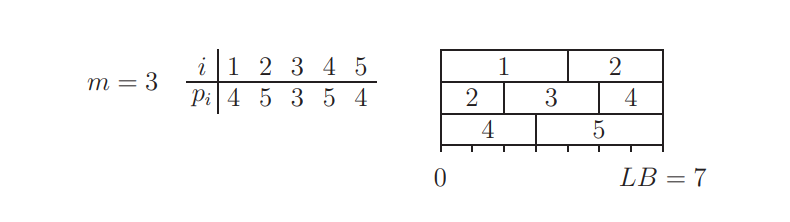
\includegraphics[width=1.1\textwidth]{imgs/mmsPTAS/pmtn-Cmax.png}
    \end{figure}
\end{frame}

\renewcommand{\subsectiontitle}{Scheduling on Unrelated Parallel Machines }
\subsection{\subsectiontitle}

\begin{frame}{\subsectiontitle}
Dado un conjunto $J$ de trabajos, un conjunto $M$ de maquinas, y por cada $j\in J$ y $i\in M$, tenemos $p_{ij}\in \mathbf{Z}^+$, que es el tiempo que se tarda en procesar el trabajo $j$ en la maquina $i$, el problema es calendarizar los trabajos en las maquinas para minimizar el makespan, es decir el tiempo de procesamiento máximo de cualquier maquina. En el libro se denota el numero de trabajos como $n$ y el numero de maquinas como $m$.\\

Nota: decimos "no relacionadas" porque no hemos supuesto ninguna relación entre los tiempos de procesamiento de un trabajo en diferentes maquinas. si cada trabajo tiene el mismo tiempo de procesamiento, sea $p_j$ dicho tiempo, en cada una de las maquinas, entonces decimos que las maquinas son \textit{identicas}.
\end{frame}

\begin{frame}{\subsectiontitle}
Para el 2-algoritmo para el problema de la programación en máquinas paralelas no relacionadas aplicaremos la técnica de poda paramétrica, junto con el redondeo de programación lineal, para obtener el algoritmo.
\end{frame}

\renewcommand{\subsectiontitle}{Poda paramétrica en una configuración de Programación Lineal}
\subsection{\subsectiontitle}

\begin{frame}{\subsectiontitle}
En este programa $x_{ij}$ es una variable indicadora que nos dice si el trabajo $j$ está programado(calendarizado) en la máquina $i$. El objetivo es minimizar $t$, el makespan. El primer conjunto de restricciones nos asegura que cada trabajo es calendarizado en una de las máquinas, y el segundo conjunto asegura que cada maquina tiene un tiempo de procesamiento de a lo más $t$.
\begin{align*}
    \texttt{minimizar } &t &\\
    \texttt{sujeto a } &\sum_{i\in M}x_{ij}=1, &j \in J\\
    &\sum_{j\in J}x_{ij}p_{ij}\leq t, &i \in M\\
    &x_{ij}\in \{0,1\}, &i \in M,j \in J\\
\end{align*}
\end{frame}

\begin{frame}{Ejemplo}
Supongamos que tenemos un solo trabajo, cuyo tiempo de procesamiento es $m$ en cada $m$ maquina. El minimo makespan es $m$. Sin embargo, la solución óptima para la relajación lineal es calendarizar el trabajo exactamente a $1/m$ en cada maquina, lo que conduce a un
valor de 1, y dando una brecha de integralidad de $m$.
\begin{figure}
        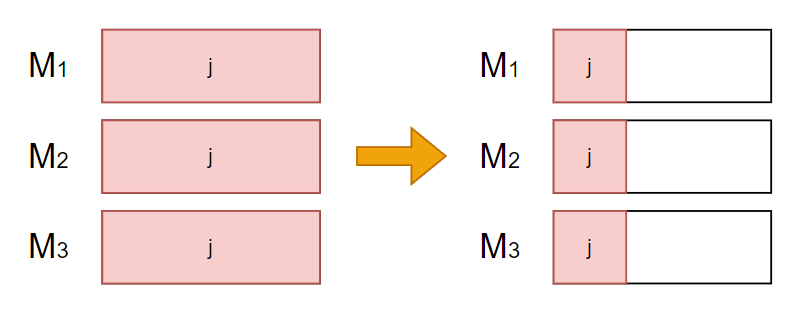
\includegraphics[width=0.8\textwidth]{imgs/mmsPTAS/ejemplojentre3.png}
    \end{figure}
\end{frame}

\begin{frame}{\subsectiontitle}
Este ejemplo ocupa una ventaja injusta que se le da por la relajación lineal. El programa entero asigna 0 a $x_{ij}$ de forma automática si $p_{ij}>t$. Pero visto de otra forma, a la relajación lineal se le tiene permitido asignar estas variables a valores que no sean 0, y de ahí obtener la solución más "barata". Esta situación podría ser rectificada si pudiéramos añadir la siguiente restricción a la relajación lineal:\\
\begin{align*}
    \forall i \in M, j\in J : \texttt{if } p_{ij}>t \texttt{ then } x_{ij} = 0.
\end{align*}
\end{frame}

\begin{frame}{\subsectiontitle}
    La restricción anterior no es una restricción lineal.\\
    Entonces para afrontar esta dificultad se usa la técnica de poda paramétrica. El parámetro será $T\in \mathbf{Z}^+$, que sera ell candidato para un limite inferior para el makespan optimo. El parámetro nos permitirá podar todos los pares máquina-trabajo tales que $p_{ij} > T$. Se define $S_T=\{(i,j)|p_{ij}\leq T\}$. Se define una familia de programas lineales $LP(T)$, una para cada valor el parámetro $T\in \mathbf{Z}^+$. $LP(T)$ usa las variables $x_{ij}$ solo para $(i,j)\in S_T$, y pregunta si hay una calendarización fraccionada y factible del makespan $\leq T$ usando las posibilidades restringidas.
    \begin{align*}
    \sum_{i:(i,j)\in S_T}x_{ij}=1, &j \in J\\
    \sum_{j:(i,j)\in S_T}x_{ij}p_{ij}\leq T, &i \in M\\
    x_{ij}\geq 0, &(i,j) \in S_T\\
\end{align*}
\end{frame}

\renewcommand{\subsectiontitle}{Propiedades de solución de punto extremo}
\subsection{\subsectiontitle}

\begin{frame}{\subsectiontitle}
Por medio de una búsqueda binaria, encontramos el valor más pequeño de $T$ tal que $LP(T)$ tiene una solución factible. Digamos que $T^*$ es este valor, $T^*$ es un limite inferior en OPT(el costo de una solución fraccionada óptima). El algoritmo redondea una solución de punto extremo a $LP(T*)$ para encontrar una calendarización con makespan $\leq 2T^*$.
\end{frame}

\begin{frame}{\subsectiontitle}
Lema 17.3: Cualquier solución de punto extremo para $LP(T)$ tiene a lo más $n+m$ variables diferentes de 0.\\

\vspace{10pt}
Demostración: Sea $r=|S_T|$ el número de variables en que $LP(T)$ está definido. Recordemos que una solución factible para $LP(T)$ es una solución de punto extremo si y sólo si corresponde a establecer $r$ restricciones linealmente independientes de $LP(T)$ para la igualdad.\\

\vspace{5pt}
De estas $r$ restricciones linealmente independientes, al menos $r-(n+m)$ deben ser elegidas a partir del tercer conjunto de restricciones (de la forma $x_{ij}\geq 0$). Las variables correspondientes se establecen con 0. Entonces, cualquier solución de punto extremo tiene a lo más $n+m$ variables distintas de 0.
\end{frame}

\begin{frame}{\subsectiontitle}
Sea $x$ una solución de punto extremo para $LP(T)$. Diremos que el trabajo $j$ es establecido de manera integral en $x$ si esta asignado de manera entera a una maquina. De otro modo diremos que $j$ está establecido de manera fraccionada.
\end{frame}

\begin{frame}{\subsectiontitle}
Corolario 17.4: Cualquier solución de punto extremo para $LP(T)$ debe establecer al menos $n-m$ trabajos de forma integral.\\

\vspace{10pt}
Demostración: Sea $x$ una solución de punto extremo para $LP(T)$, y sea $\alpha$ y $\beta$ el número de trabajos que son establecidos de manera integral y fraccionada respectivamente. Cada trabajo fraccionado está asignado al menos a 2 maquinas y así resulta en al menos 2 entradas en $x$ diferentes de 0. Así tenemos 
\begin{align*}
    \alpha + \beta = n &\alpha+2\beta \leq n+m
\end{align*}

Entonces tenemos que $\beta \leq m$ y $\alpha \geq n-m$
\end{frame}

\begin{frame}{\subsectiontitle}
    Correspondiente a una solución de punto extremo $x$ a $LP(T)$,
definimos $G = ( J, M, E)$ como la gráfica bipartita en el conjunto de vértices $J \cup M$ tal que $(j, i) \in E$ si y solo si $X_{ij} \neq 0$. Sea $F \subset J$ el conjunto de trabajos que se establecen de manera fraccionada en $x$, y sea $H$ la subgrafica de $G$ inducida en el conjunto de vértices $F\cup M$. Claramente,$( i, j )$ es una arista en $H$ si y solo si $0 < X_{ij} < 1$. Un emparejamiento en $H$ será perfecto si empareja todos los trabajos $j \in F$. El procedimiento de redondeo utiliza el hecho que la gráfica H tiene un emparejamiento perfecto.
\end{frame}

\renewcommand{\subsectiontitle}{Algoritmo de aproximación}
\subsection{\subsectiontitle}

\begin{frame}{\subsectiontitle}
\begin{enumerate}
    \item Por medio de una búsqueda binaria entre el intervalo [$\alpha/m, \alpha$], encontramos el valor más pequeño de $T\in \mathbf{Z}^+$ para el cual $LP(T)$ tiene una solución factible. Le asignamos este valor a $T^*$.%\hspace{7cm} O(nlogn)
    \item Buscamos una solución para el punto extremo, sea $x$ esta solución para $LP(T^*)$.%\hspace{6cm} O()
    \item Asignamos todos los trabajos agregados a las maquinas como con $x$.%\hspace{0.3cm} O()
    \item Construimos la gráfica $H$ y encontramos un emparejamiento perfecto $M$ en ella.%\hspace{5.1cm} O()
    \item Asignamos trabajos establecidos fraccionadamente a las máquinas acorde al emparejamiento de M.%\hspace{7.8cm} O()
\end{enumerate}
\end{frame}

\renewcommand{\subsectiontitle}{Propiedades adicionales de solución de punto extremo}
\subsection{\subsectiontitle}

\begin{frame}{\subsectiontitle}
Una gráfica conexa con su conjunto $V$ de vértices es un pseudo-arbol si contiene a lo más $|V|$ aristas. Como la gráfica es conexa tiene que tener al menos $|V|-1$ aristas. Entonces tenemos que la gráfica o es un árbol o un árbol con una arista extra. En este último caso sabemos que la gráfica tiene un solo ciclo. Digamos que una gráfica es un pseudo-bosque si cada uno de los componentes conexos de la gráfica son pseudo-arboles. 
\end{frame}

\begin{frame}{\subsectiontitle}
Lemas
\begin{enumerate}
    \item[\textbf{17.6}] La gráfica $G$ es un pseudo-bosque.
    \item[\textbf{17.7}] La gráfica $H$ tiene un emparejamiento perfecto.
    \end{enumerate}
    Teorema
    \begin{enumerate}
    \item[\textbf{17.8}] El algoritmo de aproximación nos garantiza un factor 2 para el problema de calendarizar en maquinar paralelas no relacionadas.
\end{enumerate}
\end{frame}

\begin{frame}{Lema: La gráfica $G$ es un pseudo-bosque}
Demostración:\\
En esta demostración mostramos que el número de aristas en cada componente conexo de $G$ está acotado por el número de vértices que hay en el. Entonces cada componente conexo es un pseudo-árbol.\\

\vspace{10pt}
Consideramos un componente conexo $G_C$. Restringimos $LP(T)$ y $x$ a los trabajos y maquinas de $G_C$, para obtener $LP_C(T)$ y $x_C$. Sea $x_{\overline{C}}$ el resto de $x$.\\

\vspace{5pt}
Una observación importante es que $x_C$ debe ser una solución de punto extremo para $LP_C(T)$.
\end{frame}

\begin{frame}{\subsectiontitle}
    Supongamos que este no es el caso. Entonces $x_C$ es una combinación convexa de 2 soluciones factibles para $LP_C(T)$. Cada una de estas, junto con $x_{\overline{C}}$, forman una solución factible para $LP(T)$. Así $x$ es una combinación convexa de 2 soluciones factibles para $LP(T)$. Esto nos lleva a una contradicción.\\

Aplicando el lema 17.3 (Cualquier solución de punto extremo para $LP(T)$ tiene a lo más $n+m$ variables diferentes de 0), tenemos que $G_C$ es un pseudo-árbol.
\end{frame}

\begin{frame}{Lema: H tiene emparejamiento perfecto}
Cada trabajo que se coloca en $x$ tiene exactamente una arista incidente en $G$. Eliminamos estos trabajos, junto con sus aristas incidentes, de $G$. La gráfica que nos queda es $H$. Ya que se eliminaron un mismo número de aristas y de vértices, $H$ igual es un pseudo-bosque.
\end{frame}

\begin{frame}{}
\begin{figure}
        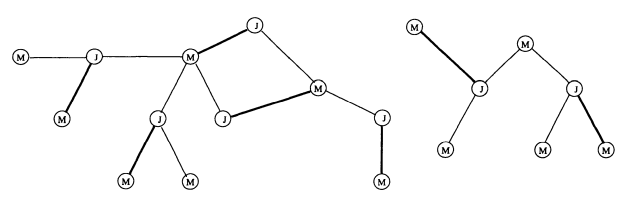
\includegraphics[width=0.9\textwidth]{imgs/mmsPTAS/graficaH.png}
    \end{figure}
\end{frame}

\begin{frame}{}
En $H$, cada trabajo tiene un grado de a lo menos 2. Entonces, todas las hojas en $H$ deben ser maquinas. Seguimos emparejando una hoja con el trabajo en el que la hoja incide, y eliminamos a ambos de la gráfica. En cada paso las hojas deben ser maquinas, al final nos quedaran ciclos pares, ya que empezamos con una gráfica bipartita. Emparejamos aristas de forma alternada en cada ciclo. Esto nos da un emparejamiento perfecto en $H$.
\end{frame}

\renewcommand{\subsectiontitle}{Garantizado factor 2 para algoritmo de aproximación}
\subsection{\subsectiontitle}

\begin{frame}{\subsectiontitle}
Demostración:\\

\vspace{10pt}
Claramente $T^*\leq$OPT, ya que $LP(OPT)$ tiene una solución factible. La solución de punto extremo, $x$, para $LP(T^*)$ tiene un makespan fraccionado $\leq T^*$. Por lo tanto, la restricción de $x$ para establecer trabajos integralmente tiene un makespan $\leq T^*$. Cada arista $(i,j)$ de $H$ satisface $p_{ij}\leq T$. El emparejamiento perfecto encontrado en $H$ calendariza a lo más un trabajo de más en cada maquina. Por lo tanto, el makespan total es $\leq 2T^* \leq 2 \cdot OPT$. El algoritmo corre en tiempo polinomial.
\end{frame}

\renewcommand{\subsectiontitle}{Ejemplo}
\subsection{\subsectiontitle}

\begin{frame}{\subsectiontitle}
Sean $m^2-m+1$ los trabajos que necesitan ser calendarizados en $m$ maquinas.
\begin{figure}
    \centering
    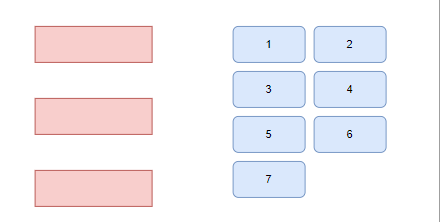
\includegraphics{imgs/mmsPTAS/EjemploMMUPM1.png}
\end{figure}
\end{frame}

\begin{frame}{\subsectiontitle}
El primer trabajo tiene un tiempo de procesamiento de $m$ en todas las maquinas, y el resto de los trabajos tienen tiempo de procesamiento unitario en cada máquina.
\begin{figure}
    \centering
    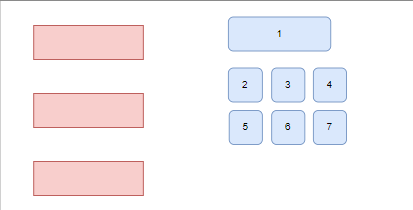
\includegraphics{imgs/mmsPTAS/EjemploMMUPM2.png}
\end{figure}
\end{frame}

\begin{frame}{\subsectiontitle}
El calendarizado optimo asigna el primer trabajo a una máquina
\begin{figure}
    \centering
    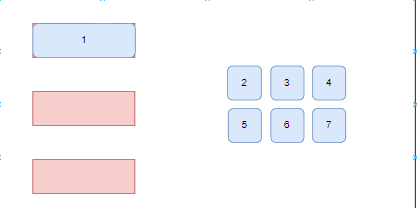
\includegraphics{imgs/mmsPTAS/EjemploMMUPM3.png}
\end{figure}
\end{frame}

\begin{frame}{\subsectiontitle}
y a los $m$ trabajos restantes a cada $m-1$ máquinas restantes.
\begin{figure}
    \centering
    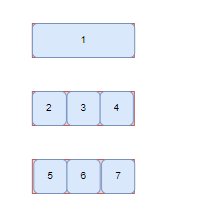
\includegraphics{imgs/mmsPTAS/EjemploMMUPM4.png}
\end{figure}
 El makespan es $m$. Es fácil ver que $LP(T)$ no tiene una solución factible para $T<m$.
\end{frame}

\begin{frame}{\subsectiontitle}
Ahora suponemos que la siguiente solución de punto extremo para $LP(T)$ es elegida. Asigna $1/m$ al primer trabajo
\begin{figure}
    \centering
    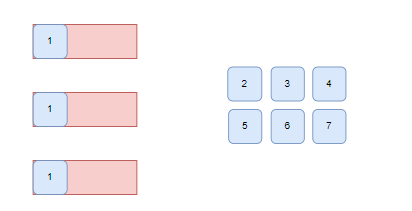
\includegraphics{imgs/mmsPTAS/EjemploMMUPM5.png}
\end{figure} y $m-1$ a los demás trabajos a cada una de las $m$ maquinas.\\

El redondeo producirá una calendarización con un makespan de $2m-1$.
\end{frame}


\begin{frame}{\subsectiontitle}
y $m-1$ a los demás trabajos a cada una de las $m$ maquinas.
\begin{figure}
    \centering
    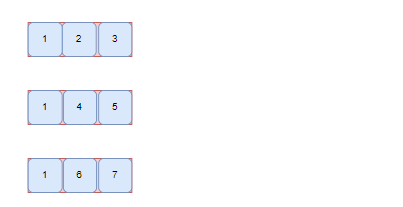
\includegraphics{imgs/mmsPTAS/EjemploMMUPM6.png}
\end{figure} 
El redondeo producirá una calendarización con un makespan de $2m-1$.
\end{frame}